%% ============================================================================
%%  WATER LEAK LOCALIZATION SYSTEM (LeakLens)
%%  Project report in the IIIT Kottayam thesis format (BTP Phase 1, Review 2)
%%  Compile with:  tectonic main.tex   (or  pdflatex main.tex  twice)
%% ============================================================================
\documentclass[11pt,letterpaper]{report}

\usepackage[letterpaper,left=1.55in,right=1.55in,top=1.5in,bottom=1.6in]{geometry}
\usepackage[T1]{fontenc}
\usepackage{amsmath,amssymb,amsthm}
\usepackage{graphicx}
\usepackage{booktabs,array,tabularx,longtable}
\usepackage{float}
\usepackage[font=small]{caption}
\usepackage{enumitem}
\usepackage{listings}
\usepackage{tikz}
\usetikzlibrary{arrows.meta,positioning}
\usepackage[hidelinks]{hyperref}

\newcolumntype{Y}{>{\raggedright\arraybackslash}X}
\setlist{itemsep=2pt,topsep=3pt}

% ---- theorem-like environments, numbered inside sections (1.1.1, 1.1.2, ...) --
\theoremstyle{definition}
\newtheorem{theorem}{Theorem}[section]
\newtheorem{definition}[theorem]{Definition}
\theoremstyle{plain}
\newtheorem{proposition}[theorem]{Proposition}
\newtheorem{corollary}[theorem]{Corollary}
\theoremstyle{remark}
\newtheorem{remark}[theorem]{Remark}

\lstset{basicstyle=\ttfamily\footnotesize,breaklines=true,frame=single,columns=fullflexible,xleftmargin=2pt,xrightmargin=2pt}
\newcommand{\code}[1]{\texttt{#1}}
\newcommand{\LL}{LeakLens}

\linespread{1.3}

\begin{document}
\pagenumbering{roman}

%% ------------------------------------------------------------------ TITLE PAGE
\thispagestyle{empty}
\begin{center}
\linespread{1.15}\selectfont
\vspace*{-0.2in}
{\large\bfseries WATER LEAK LOCALIZATION SYSTEM}\\[0.15in]
{\normalsize\bfseries(LeakLens: Detecting, Classifying and Localizing Leaks\\ in Water Distribution Networks)}

\vspace{0.3in}
{\small A Project Report Submitted\\ in Partial Fulfilment of the Requirements\\ for the Degree of}\\[0.18in]
{\large\bfseries BACHELOR OF TECHNOLOGY}\\[0.08in]
{\small\itshape by}\\[0.08in]
{\normalsize\bfseries Ashish Ranjan (Roll No.\ 2023BCS0027)\\
Nidamanuri Kedar Vaishnav (Roll No.\ 2023BCS0163)\\
Abhinandh Rajeev (Roll No.\ 2023BCS0074)\\
Kadthala Hrishith Reddy (Roll No.\ 2023BCS0168)}\\[0.15in]
{\small Under the Supervision of}\\[0.05in]
{\normalsize\bfseries Dr.\ Divya Sindhu Lekha}

\vspace{0.2in}

\includegraphics[width=2.0in]{figures/logo.jpg}

\vspace{0.2in}
{\normalsize\bfseries DEPARTMENT OF COMPUTER SCIENCE AND ENGINEERING\\
INDIAN INSTITUTE OF INFORMATION TECHNOLOGY\\
KOTTAYAM-686635, INDIA}\\[0.1in]
{\small\itshape October 2026}
\end{center}
\clearpage

%% ------------------------------------------------------------------ DECLARATION
\begin{center}\vspace*{0.7in}{\large\bfseries DECLARATION}\end{center}
\vspace{0.15in}
{\linespread{1.6}\selectfont
We, \textbf{Ashish Ranjan} (\textbf{Roll No: 2023BCS0027}), \textbf{Nidamanuri Kedar Vaishnav} (\textbf{Roll No: 2023BCS0163}), \textbf{Abhinandh Rajeev} (\textbf{Roll No: 2023BCS0074}) and \textbf{Kadthala Hrishith Reddy} (\textbf{Roll No: 2023BCS0168}), hereby declare that this report entitled \textbf{``Water Leak Localization System''} submitted to Indian Institute of Information Technology Kottayam towards partial requirement of \textbf{Bachelor of Technology} in \textbf{Computer Science and Engineering} is an original work carried out by us under the supervision of \textbf{Dr.\ Divya Sindhu Lekha} and has not formed the basis for the award of any degree or diploma, in this or any other institution or university. We have sincerely tried to uphold the academic ethics and honesty. Whenever an external information or statement or result is used then, that have been duly acknowledged and cited.
}
\vspace{1.1in}

\noindent Kottayam-686635 \hfill \textbf{Ashish Ranjan}\\
October 2026 \hfill \textbf{Nidamanuri Kedar Vaishnav}\\
\mbox{} \hfill \textbf{Abhinandh Rajeev}\\
\mbox{} \hfill \textbf{Kadthala Hrishith Reddy}
\clearpage

%% ------------------------------------------------------------------ CERTIFICATE
\begin{center}\vspace*{0.7in}{\large\bfseries CERTIFICATE}\end{center}
\vspace{0.15in}
{\linespread{1.6}\selectfont
This is to certify that the work contained in this project report entitled \textbf{``Water Leak Localization System''} submitted by \textbf{Ashish Ranjan} (\textbf{Roll No: 2023BCS0027}), \textbf{Nidamanuri Kedar Vaishnav} (\textbf{Roll No: 2023BCS0163}), \textbf{Abhinandh Rajeev} (\textbf{Roll No: 2023BCS0074}) and \textbf{Kadthala Hrishith Reddy} (\textbf{Roll No: 2023BCS0168}) to the Indian Institute of Information Technology Kottayam towards partial requirement of \textbf{Bachelor of Technology} in \textbf{Computer Science and Engineering} has been carried out by them under my supervision and that it has not been submitted elsewhere for the award of any degree.
}
\vspace{0.9in}

\noindent Kottayam-686635 \hfill (Dr.\ Divya Sindhu Lekha)\\
October 2026 \hfill Project Supervisor

\vspace{0.9in}
\begin{flushright}
(Dr.\ [Name of the Head of the Department])\\
Head of the Department\\
Dept.\ of Computer Science \& Engineering
\end{flushright}
\clearpage

%% ------------------------------------------------------------------ ABSTRACT
\begin{center}\vspace*{0.7in}{\large\bfseries ABSTRACT}\end{center}
\vspace{0.1in}
\linespread{1.3}\selectfont
Water distribution networks lose a large share of treated water to leaks, but a pressure drop alone does not prove a leak: a hydrant opening, a pump stopping or a tank running low lowers the pressure as well. The main aim of this project is therefore to build a software system that, from pressure, pipe-flow and customer-demand data, decides whether a network is behaving normally, names the kind of event (leak, demand change, pump or reservoir change, tank change, blocked pipe, pipe ageing) and, for a leak, ranks the junctions where it most probably is.

The work is carried out on simulated data. A scenario generator built on EPANET and WNTR produces 617 labelled 24-hour scenarios on three benchmark networks, covering leaks of five sizes at every junction and four start times, demand changes, hydrant flow, pump outages, reservoir and tank changes, blocked pipes, pipe ageing, sensor noise and leaks hidden behind other events. The method learns the sensor-noise level of each network, computes \emph{unaccounted flow} (water that leaves a node without a customer meter recording it), summarises each scenario into fourteen features and uses a random forest to name the event. A fixed score, unaccounted flow plus a weighted pressure drop, ranks the junctions. The system is delivered through a FastAPI backend with an SQLite scenario catalogue and a Next.js dashboard with light and dark themes.

All scenarios were split once into 478 for learning and 139 for testing; every result is measured on the unseen test scenarios. The exact leak junction is ranked first for 96.7\% of the test leaks (the first prototype: 58.3\%), the real junction is among the first five for 98.3\%, false alarms on normal days fall from 41.7\% to 0.0\%, and the kind of event is named correctly for 82.7\% of the test scenarios. We report where the method fails: leaks inside the sensor noise, the largest leaks, and telling pump, tank, blockage and ageing events apart on a network not seen in training. All results are from simulation, not real sensors.
\clearpage

%% ------------------------------------------------------------------ ACKNOWLEDGMENT
\begin{center}\vspace*{0.7in}{\large\bfseries ACKNOWLEDGMENT}\end{center}
\vspace{0.1in}
We express our sincere gratitude to our project supervisor, \textbf{Dr.\ Divya Sindhu Lekha}, for her guidance, encouragement and constructive criticism throughout this project. Her suggestions on how to make the evaluation honest, in particular to separate the data used for learning from the data used for testing, shaped this report.

We thank the Head of the Department and the faculty of the Department of Computer Science and Engineering, Indian Institute of Information Technology Kottayam, for the facilities and the academic environment that made this work possible. We also thank the developers of the open-source tools on which the project stands, namely EPANET, WNTR, scikit-learn, FastAPI and Next.js, and the authors of the papers cited in this report. Finally, we thank our families and friends for their constant support.
\clearpage

%% ------------------------------------------------------------------ CONTENTS
\tableofcontents
\clearpage
\addcontentsline{toc}{chapter}{List of Figures}
\listoffigures
\clearpage
\addcontentsline{toc}{chapter}{List of Tables}
\listoftables
\clearpage
\pagenumbering{arabic}

%% ================================================================ CHAPTER 1
\chapter{Introduction}
Water distribution networks (WDNs) carry treated water from sources to customers through pipes, pumps, tanks and valves. Part of that water never reaches a customer because pipes leak. This chapter explains why leak localization matters, states the problem, lists the objectives and contributions of the project, and describes how the rest of the report is organised.

\section{Motivation and Background}
Water utilities lose a large share of the water they produce through leaks and other unmetered use, usually called non-revenue water. The literature reports leakage from about 3\% to over 50\% depending on maintenance \cite{sousa2026review}, and our project presentation quotes about 40\% for developing countries. Leaks waste water and energy, damage roads and buildings and can let contamination enter the pipes.

Finding leaks by inspecting streets or listening to pipes with acoustic equipment is slow and labour-intensive \cite{vaquet2024survey}. Pressure and flow sensors scale better to large networks, but a pressure drop alone is ambiguous. A hot day, a hydrant, a stopped pump or a tank running low also lowers pressure, so a fixed pressure alarm either misses leaks or raises many false alarms. Software methods that combine a hydraulic model with data analysis are therefore considered a promising direction \cite{sousa2026review,romeroben2023review}.

\section{Problem Statement}
Given pressure at nodes, flow in pipes and, where available, customer demand at nodes, for a water network whose layout is known, the system must (i) decide whether the network is behaving abnormally, (ii) decide what kind of event it is, and (iii) if it is a leak, rank the candidate nodes and report the most probable location with supporting evidence.

\begin{definition}[Leak localization task]\label{def:task}
Let $\mathcal V$ be the set of junctions of a network and $\mathcal D$ the observed pressure, flow and demand time series of one day. A \emph{localizer} is a function that maps $\mathcal D$ to an ordered list of the junctions in $\mathcal V$. It is \emph{correct at rank $k$} if the true leak junction is among the first $k$ entries.
\end{definition}

\section{Objectives}
The objectives set in the project proposal for Semester~1 were to select one or two representative networks, generate normal and single-leak scenarios varying leak location, size and start time, build datasets with ground truth, establish an interpretable localization baseline, and provide a web prototype. Because the relevance of a leak detector depends on telling a leak from other hydraulic changes, the work was extended with the following objectives:
\begin{enumerate}
\item generate scenarios on three networks, including demand, pump, reservoir, tank, blockage, ageing and sensor-noise scenarios;
\item replace the fixed pressure alarm by a detector that learns the noise level of each network;
\item classify the cause of an event, not only detect it;
\item localize leaks with a method whose error is measured as distance on the pipe graph;
\item evaluate honestly on scenarios that were not used for learning;
\item deliver the result as an easy-to-use web dashboard.
\end{enumerate}

\section{Contributions and Scope}
The contribution of this project is the \emph{integration} of known ingredients and a controlled, reproducible study; it does not claim a new algorithm. In particular:
\begin{itemize}
\item a reproducible scenario generator with ground truth on three benchmark networks;
\item a noise-aware detector with a two-hour persistence rule and a quiet check;
\item a cause classifier built on fourteen physics-based features;
\item a localizer based on \emph{unaccounted flow}, whose error is measured in pipe hops and metres;
\item an 80/20 hold-out evaluation in which near-copies of a scenario stay on the same side of the split;
\item a FastAPI backend with an SQLite catalogue and a Next.js dashboard with light and dark themes.
\end{itemize}
The scope is limited to simulated data, single leaks, and demand measured at every node. Missing or sparse sensors, multiple simultaneous leaks and real utility data are left for Semester~2.

\section{Organisation of the Report}
Chapter~2 reviews related work. Chapter~3 gives the hydraulic background and the governing equations. Chapter~4 describes the networks, scenarios and data. Chapter~5 presents the method. Chapter~6 describes the implementation of the backend and dashboard. Chapter~7 gives the evaluation protocol and results. Chapter~8 concludes and outlines future work.

%% ================================================================ CHAPTER 2
\chapter{Literature Review and Related Work}
This chapter surveys recent work on leak detection and localization in water distribution networks and positions the project against it. Reviews and benchmarks are covered first, then data-driven methods trained on simulated data, graph and topology-based methods, and work on classifying anomalies.

\section{Reviews and Benchmarks}
Sousa et al.\ \cite{sousa2026review} review scientific, industrial and commercial developments in leakage management, compare hardware-based, software-based and hybrid techniques, and report trade-offs in scalability, data dependency, uncertainty and localization accuracy. Romero-Ben et al.\ \cite{romeroben2023review} review the move from model-based to data-based leak localization and compare promising methods on a benchmark. Vaquet et al.\ \cite{vaquet2024survey} survey machine learning in water distribution networks, including a structured review of leakage detection and localization and evaluation benchmarks.

Benchmarks make comparison possible. LeakDB \cite{vrachimis2018leakdb} provides simulated but realistic leakage scenarios built with WNTR. The Battle of the Leakage Detection and Isolation Methods (BattLeDIM) compared methods on a virtual network with SCADA measurements and concluded that further development of methods and additional open benchmark problems are needed \cite{vrachimis2022battledim}.

\section{Data-Driven Methods Trained on Simulated Leaks}
Because real leaks seldom come with ground truth, many methods are trained on hydraulic simulations. Lu\v{c}in et al.\ \cite{lucin2021rf} train a random forest on simulated leaks with random location, size and demand uncertainty from pressure sensors, and add pipe segmentation so that the leak is located along a pipe and not only at a node. Marvin et al.\ \cite{marvin2023hgb} generate pressure data with randomly varied leak location, area and start time, add pressure noise, and compare a random forest with histogram-based gradient boosting, which performs better. Basnet et al.\ \cite{basnet2023supervised} study supervised multilayer-perceptron and convolutional models for localization under different leak complexities on a benchmark network. Rajabi et al.\ \cite{rajabi2023cdcgan} turn pressure data into images by kriging interpolation and use a conditional generative adversarial network for detection and localization.

These studies motivate our use of simulated, labelled scenarios and a tree-based classifier, and they show that random forests and gradient boosting are common choices for this tabular problem.

\section{Hybrid, Graph and Topology-Based Methods}
Soldevila et al.\ \cite{soldevila2022hybrid} combine expert knowledge with data-driven models: leaks are detected on the inlet flow and localized by a classifier that groups locations the sensors cannot tell apart; it is evaluated on one network. Irofti et al.\ \cite{irofti2021dictionary} combine graph-based interpolation with dictionary-learning classification on the L-Town benchmark. Leonzio et al.\ \cite{leonzio2026centrality} select monitoring nodes with graph centrality and show that the sensor strategy that works best depends on topology. Zhang and Fink \cite{zhang2026aignn} pre-train a graph neural network to imitate a max-flow algorithm so that it generalizes better, and van Gemert et al.\ \cite{vangemert2026sensorplacement} study how sensor placement affects graph-neural-network leak detection.

\section{Classifying the Kind of Anomaly}
Most localization studies assume that a leak is the only possible event. Melnikov et al.\ \cite{melnikov2025sicams} are closer to our question: they test whether a network behaves normally with a statistical method, classify anomalies as abrupt leaks, incipient leaks or sensor malfunctions, and give a coarse pre-localization. Our work extends the set of alternatives to demand changes, pump and reservoir changes, tank changes, blocked pipes and pipe ageing.

\section{Comparison and Research Gap}
\begin{table}[H]
\centering\small
\caption{Summary of related work and positioning of this project.}\label{tab:related}
\begin{tabularx}{\textwidth}{@{}p{1.1in}YY@{}}
\toprule
Work & Approach and data & Main limitation \\
\midrule
Lu\v{c}in et al.\ 2021 \cite{lucin2021rf} & Random forest on simulated leaks, pipe segmentation & Leak is the only event considered \\
Marvin et al.\ 2023 \cite{marvin2023hgb} & Gradient boosting vs.\ random forest, WNTR data & Single network; leak only \\
Basnet et al.\ 2023 \cite{basnet2023supervised} & MLP and CNN on L-Town & Leak only; black-box models \\
Soldevila et al.\ 2022 \cite{soldevila2022hybrid} & Inlet-flow test and clustered classifier & One network; no graph reasoning \\
Leonzio et al.\ 2026 \cite{leonzio2026centrality} & Centrality-guided sensor selection, autoencoder & Detection, not localization \\
Zhang and Fink 2026 \cite{zhang2026aignn} & Algorithm-informed graph neural network & Learned; hard to interpret \\
Melnikov et al.\ 2025 \cite{melnikov2025sicams} & Multivariate statistics; anomaly classes & Coarse localization; preprint \\
\textbf{This project} & Noise-aware detection, unaccounted flow, random forest, ranking; three networks & Simulation only; demand meters assumed \\
\bottomrule
\end{tabularx}
\end{table}
The studies above typically evaluate one network at a time, treat detection and localization separately, or rely on models that are hard to explain. We did not find a work that combines noise-aware detection, flow-balance reasoning, classification of the kind of event, a graph-distance error measure and an interpretable ranked output with an evaluation on held-out scenarios across networks. Our search was not exhaustive.

%% ================================================================ CHAPTER 3
\chapter{Hydraulic Background}
This chapter introduces the hydraulic concepts and equations used to generate the data and to interpret it.

\section{Water Distribution Networks as Graphs}
A network is a graph whose vertices are \emph{junctions} (where customers draw water), \emph{reservoirs} (sources with fixed head) and \emph{tanks} (storage), and whose edges are \emph{pipes}, \emph{pumps} and \emph{valves}. Every edge has a start and an end node, and the flow in it is signed: positive from start to end.

\begin{definition}[Pressure, flow and demand]\label{def:pfd}
The \emph{pressure} $P_i(t)$ at node $i$ and hour $t$ is the pressure head in metres. The \emph{flow} $Q_p(t)$ is the volume of water passing pipe $p$ per second (m$^3$/s). The \emph{demand} $D_i(t)$ is the water delivered to the customers of node $i$ (m$^3$/s).
\end{definition}

\section{EPANET and WNTR}
EPANET \cite{epanet} is the standard hydraulic simulator for pressurised pipe networks and defines the \texttt{.inp} network format. WNTR \cite{wntr} is a Python package that loads such files and adds leaks, controls, demand patterns and pump outages, and it provides its own simulator. We use WNTR's simulator with \emph{pressure-dependent demand} (PDD): when pressure is low, the delivered demand falls below the requested demand. This is more realistic than demand-driven analysis for leaks and pump outages.

\section{Governing Equations}
\begin{definition}[Continuity at a junction]\label{def:balance}
For a junction $i$, let $\operatorname{sign}(p,i)=+1$ if pipe $p$ ends at $i$ and $-1$ if it starts there. The \emph{net inflow} is
\begin{equation}
\mathrm{div}_i(t)=\sum_{p}\operatorname{sign}(p,i)\,Q_p(t).
\end{equation}
Conservation of mass requires
\begin{equation}\label{eq:balance}
\mathrm{div}_i(t)=D_i(t)+Q_{\ell,i}(t),
\end{equation}
where $Q_{\ell,i}$ is the leak flow at node $i$ ($0$ if there is no leak).
\end{definition}

A leak is modelled as an orifice. With discharge coefficient $C_d=0.75$, hole area $A$, gravitational acceleration $g=9.81$ m/s$^2$ and pressure head $P_i$,
\begin{equation}\label{eq:orifice}
Q_{\ell,i}(t)=C_d\,A\,\sqrt{2\,g\,P_i(t)}\qquad (t\ge t_{\text{start}}),
\end{equation}
so the leak flow grows with the pressure. Customer demand is the base demand scaled by a daily pattern and a scenario factor,
\begin{equation}\label{eq:demand}
D_i(t)=D_{\text{base},i}\;m(t)\;f .
\end{equation}
The pressure lost in a pipe of length $L$, diameter $d$ and roughness coefficient $C$ carrying flow $Q$ follows the Hazen--Williams law,
\begin{equation}\label{eq:hw}
h_f=\frac{10.67\,L\,Q^{1.852}}{C^{1.852}\,d^{4.87}} ,
\end{equation}
so a smaller $C$ (an older, rougher pipe) loses more pressure for the same flow.

\section{Effect of Events on the Hydraulic State}
\begin{table}[H]
\centering\small
\caption{What each kind of event does to the network.}\label{tab:effects}
\begin{tabularx}{\textwidth}{@{}p{0.95in}YYp{0.8in}@{}}
\toprule
Event & Pressure & Flow balance & Water lost? \\
\midrule
Leak & Largest drop at one node, decaying with distance & Unmetered loss at that node & Yes \\
Demand change & Drop near heavy use & Extra flow is metered & No \\
Pump / reservoir & Wide drop or shift over the served area & Pump flow falls; tanks supply & No \\
Tank change & Shift near the tank & Tank flow changes sign or size & No \\
Blocked pipe & Down downstream, may rise upstream & Flow reroutes & No \\
Pipe ageing & Slow, wide loss, largest where flow is high & No node imbalance & No \\
\bottomrule
\end{tabularx}
\end{table}
A leak is therefore \emph{local} and \emph{unmetered}; the other events are either metered or spread over many nodes. This difference is the basis of the method of Chapter~5.

%% ================================================================ CHAPTER 4
\chapter{Data Generation}
\section{The Networks}
Three standard EPANET benchmark networks of different size and structure are used, so that generalization can be tested.
\begin{table}[H]
\centering\small
\caption{The three benchmark networks.}\label{tab:networks}
\centering\setlength{\tabcolsep}{4pt}
\begin{tabular}{@{}lrrrrrrr@{}}
\toprule
Network & Junctions & Analysed & Pumps & Tanks & Reservoirs & Scenarios & $\tau_P$ (m) \\
\midrule
NET1 & 9 & 9 & 1 & 1 & 1 & 155 & 0.498 \\
NET2 & 35 & 35 & 0 & 1 & 0 & 171 & 0.535 \\
NET3 & 92 & 90 & 2 & 3 & 2 & 291 & 0.582 \\
\bottomrule
\end{tabular}
\end{table}
Net2 has no reservoir and no pump; one junction with negative demand acts as its supply. Net3 nodes 61 and 601 and the hour 21:00 are ignored (Section~\ref{sec:ill}).

\section{Scenario Design}
\begin{definition}[Scenario]
A \emph{scenario} is one 24-hour simulation of a network in which one thing (or a few things together) differs from the normal day. The \emph{baseline} is the normal day with nothing changed. Each scenario is stored with its \emph{true answer}, namely the kind of event and, for leaks, the leak node. The true answer is used only to label training data and to score results.
\end{definition}
Table~\ref{tab:scenarios} lists the 617 scenarios.
\begin{table}[H]
\centering\small
\caption{The scenario kinds and what is changed.}\label{tab:scenarios}
\begin{tabularx}{\textwidth}{@{}p{0.85in}p{0.45in}Y@{}}
\toprule
Kind & Count & What is changed \\
\midrule
Leak & 299 & Hole at one junction; areas 0.0001, 0.0003, 0.001, 0.003, 0.01 m$^2$ (tiny to burst); every junction; start at 2, 8, 12 or 20 h; sensor noise; hidden behind a global demand surge, a hydrant, a closed pipe or a pump outage \\
Demand change & 60 & One node $\times1.5$ or $\times0.5$; all nodes $\times1.3$ or $\times0.7$; a hydrant of 0.01 m$^3$/s for four hours \\
Pump / reservoir & 54 & A pump off for 2, 4 or 6 h while it normally runs; reservoir head $\pm2,\pm5,\pm10$ m \\
Tank change & 60 & A tank starts 10--90\% full, or its pipe is closed at 10:00 \\
Blocked pipe & 48 & A busy pipe closed from 10:00, or throttled \\
Pipe ageing & 42 & Roughness coefficient $C$ multiplied by 0.6--0.95 \\
Normal day & 54 & Nothing changes; sensor noise only (or none) \\
\bottomrule
\end{tabularx}
\end{table}
Most non-leak scenarios also have a noisy twin. The scenarios for each network are generated from the network's own layout, so every node, pipe, pump, tank and reservoir identifier is valid for that network; blockage candidates are tested for hydraulic convergence before they are included.

\section{Recorded Data and Sensor Noise}
For every scenario three tables are saved with one row per hour (hours 0 to 24): pressure at every node, flow in every pipe, and the demand delivered at every node (what a customer meter would read; the leak flow is not included). In noisy scenarios Gaussian errors with fixed random seeds are added to the saved readings: low noise is $0.05$ m on pressure and 0.5\% on flows and demands; high noise is $0.2$ m and 2\%. The baseline is kept clean because it stands for the expectation of the hydraulic model.

\section{Ill-Conditioned Nodes and Hours}\label{sec:ill}
A tiny 1\% demand probe is simulated on each network. A node whose pressure swings by more than 5 m, and an hour at which 90\% of the nodes swing by more than 0.5 m, are \emph{ill-conditioned}: they are artefacts of pump switching and not reliable signals. They are ignored in all analysis. In Net3 these are the nodes 61 and 601 (the outlet of a pump that is off) and the hour 21:00. Leaks at these nodes are therefore not scored. Scenarios whose hydraulics did not converge were discarded (three Net3 blockage candidates).

%% ================================================================ CHAPTER 5
\chapter{Methodology}
\section{Overview}
The method has two stages. Stage~1 decides whether anything is above the sensor noise. Stage~2 decides what kind of event it is and, for a leak, where. Figure~\ref{fig:pipeline} shows the flow.
\begin{figure}[H]
\centering
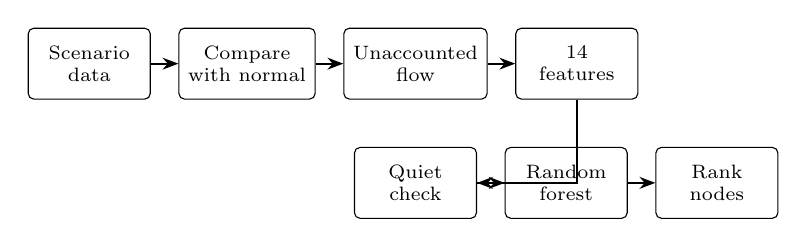
\begin{tikzpicture}[node distance=3.5mm,
 box/.style={draw,rounded corners=2pt,minimum width=1.55cm,minimum height=0.9cm,align=center,font=\scriptsize},
 arr/.style={-{Stealth[length=2mm]},thick}]
\node[box](a){Scenario\\data};
\node[box,right=of a](b){Compare\\with normal};
\node[box,right=of b](c){Unaccounted\\flow};
\node[box,right=of c](d){14\\features};
\node[box,below=6mm of c](e){Quiet\\check};
\node[box,right=of e](f){Random\\forest};
\node[box,right=of f](g){Rank\\nodes};
\draw[arr](a)--(b);\draw[arr](b)--(c);\draw[arr](c)--(d);\draw[arr](d.south)|-(e.east);\draw[arr](e)--(f);\draw[arr](f)--(g);
\end{tikzpicture}
\caption{Flow of the analysis of one scenario.}\label{fig:pipeline}
\end{figure}

\section{Residuals and Persistence}
Let $P^0_i(t)$ and $P^1_i(t)$ be the pressure of node $i$ at hour $t$ on the normal day and in the scenario. The \emph{residual} is $r_i(t)=P^0_i(t)-P^1_i(t)$; a positive residual means the pressure is lower than normal. To ignore one-off errors a change counts only if it lasts two consecutive hours.
\begin{definition}[Persistent peak]\label{def:peak}
For a series $x(t)$ the \emph{persistent peak} is
\begin{equation}
\operatorname{peak}(x)=\max_t\ \min\{x(t),\,x(t{+}1)\}.
\end{equation}
\end{definition}
\begin{remark}
For the series $0.1,\,0.2,\,6.5,\,6.7,\,6.6,\,6.4,\,0.3$ the pairwise minima are $0.1,0.2,6.5,6.6,6.4,0.3$ and the persistent peak is $6.6$. A single one-hour spike of $9.0$ between $0.2$ and $0.3$ has a persistent peak of only $0.3$.
\end{remark}

\section{Learning the Noise Level}\label{sec:noise}
Each network has normal runs that contain only sensor noise. The noise levels are learned only from the \emph{training} normal runs (14 per network). The pressure threshold is
\begin{equation}\label{eq:tau}
\tau_P=\max\{0.1\ \text{m},\;4\,\sigma_P\},
\end{equation}
where $\sigma_P$ is the standard deviation of the pressure residuals over the analysed nodes and hours. The noise levels of each pipe flow ($\sigma_{f,p}$), each node demand ($\sigma_{D,i}$) and each node's unaccounted flow ($\sigma_{a,i}$) are learned in the same way. The learned values are $\tau_P=$0.50, 0.53 and 0.58~m for Net1, Net2 and Net3.
\begin{definition}[Noise unit]
A \emph{noise unit} expresses a measurement as a multiple of its learned noise limit, so $1$ means ``exactly at the noise limit''. The pressure drop of node $i$ and its rise are
\begin{equation}
d_i=\frac{\max\{0,\operatorname{peak}(r_i)\}}{\tau_P},\qquad g_i=\frac{\max\{0,\operatorname{peak}(-r_i)\}}{\tau_P}.
\end{equation}
\end{definition}

\section{Unaccounted Flow}\label{sec:unacc}
\begin{definition}[Unaccounted flow]\label{def:unacc}
Let $\Delta$ denote the scenario value minus the normal-day value. The \emph{unaccounted flow} of node $i$ is the change in net inflow minus the change in metered demand,
\begin{equation}\label{eq:unacc}
a_i(t)=\Delta\,\mathrm{div}_i(t)-\Delta D_i(t).
\end{equation}
In noise units it is $a_i=\max\{0,\operatorname{peak}(a_i(t))\}/(4\,\sigma_{a,i})$.
\end{definition}
\begin{proposition}\label{prop:unacc}
In noise-free data, $a_i(t)=Q_{\ell,i}(t)$: the unaccounted flow of a node equals its leak flow, and it is $0$ at every node without a leak.
\end{proposition}
\begin{proof}
By continuity (\ref{eq:balance}), $\mathrm{div}_i=D_i+Q_{\ell,i}$ in the scenario and $\mathrm{div}_i=D_i$ on the normal day (no leak). Subtracting, $\Delta\mathrm{div}_i=\Delta D_i+Q_{\ell,i}$. Substituting into (\ref{eq:unacc}) gives $a_i=Q_{\ell,i}$. If node $i$ has no leak then $Q_{\ell,i}=0$ and so $a_i=0$.
\end{proof}
\begin{corollary}
A change in customer demand alone gives $a_i=0$, because the metered change $\Delta D_i$ cancels the extra net inflow. A demand change is therefore never mistaken for a leak when demands are metered.
\end{corollary}
\begin{remark}
Without nodal demand meters the second term of (\ref{eq:unacc}) is unavailable; a demand change then appears as unaccounted flow and may be mistaken for a small leak. We measure this effect in Chapter~7.
\end{remark}
\begin{figure}[H]
\centering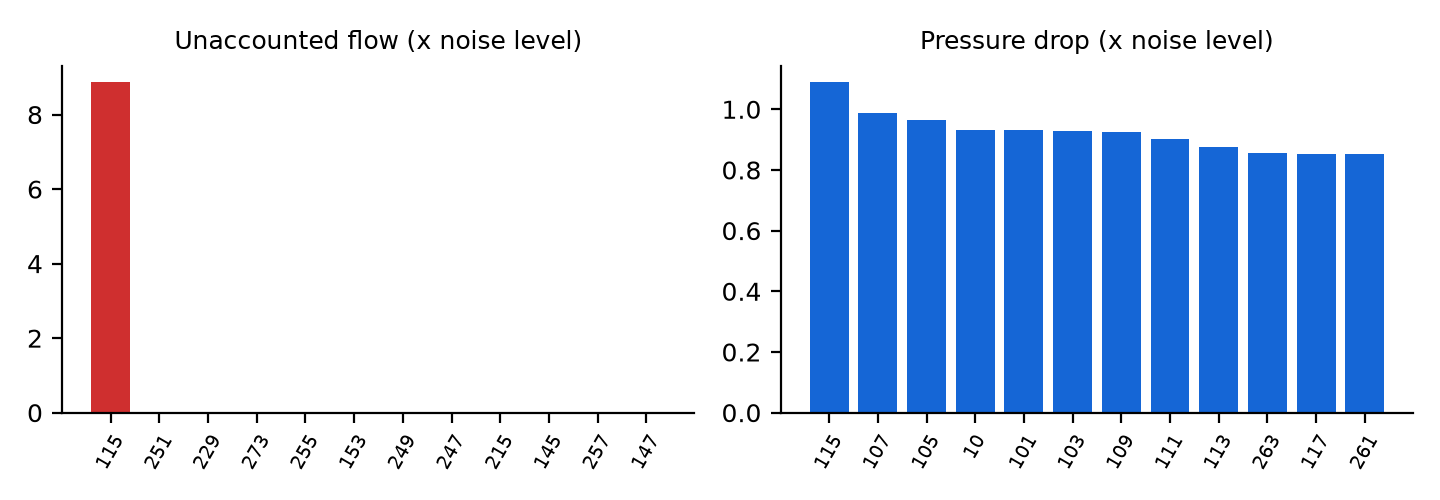
\includegraphics[width=\textwidth]{figures/fig_signals.png}
\caption{A leak at one Net3 node. Left: unaccounted flow is large at the leak node and nearly zero elsewhere. Right: the pressure drop is also high at its neighbours, so pressure alone is less precise.}\label{fig:signals}
\end{figure}
\begin{figure}[H]
\centering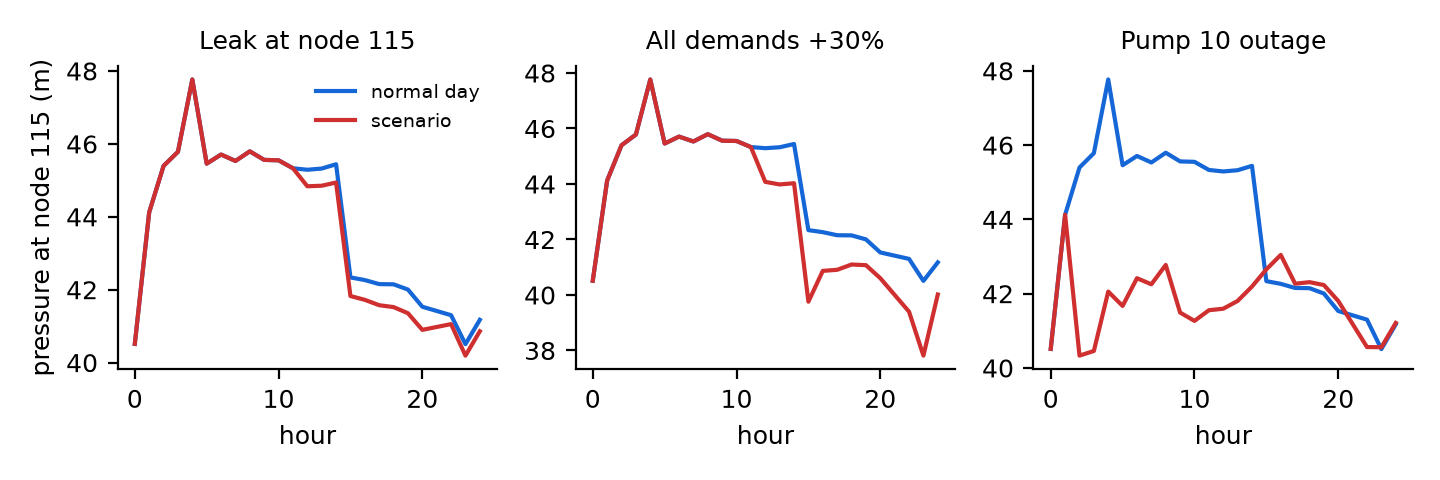
\includegraphics[width=\textwidth]{figures/fig_pressure.png}
\caption{Pressure at one Net3 node on a normal day (blue) and in three scenarios (red): a leak, a demand surge and a pump outage.}\label{fig:pressure}
\end{figure}

\section{The Fourteen Features}\label{sec:features}
Each scenario is summarised by fourteen numbers computed from the node and pipe signals of the \emph{whole network}. Here $z_p=\operatorname{peak}|Q^1_p-Q^0_p|/(4\sigma_{f,p})$ is the flow change of pipe $p$ in noise units, $z^D_i$ the same for node demands, $\Delta S(t)$ the change in total reservoir supply, $\Delta T(t)$ the change in net tank flow, $D_{tot}$ the mean total customer demand and $k$ runs over pumps.
\begin{table}[H]
\centering\footnotesize
\caption{The fourteen features of a scenario.}\label{tab:features}
\begin{tabularx}{\textwidth}{@{}p{0.2in}p{1.0in}Yp{1.45in}@{}}
\toprule
\# & Name & Meaning & Formula \\
\midrule
1 & \texttt{drop\_ratio} & Largest pressure drop at any junction & $\max_i d_i$ \\
2 & \texttt{frac\_hit} & Share of junctions that lost pressure & $\operatorname{mean}(d_i>1)$ \\
3 & \texttt{median\_ratio} & Typical (median) junction drop & $\operatorname{median}_i d_i$ \\
4 & \texttt{conc\_drop} & Is the drop concentrated at one node? & $\max d_i/\sum d_i$ \\
5 & \texttt{rise\_ratio} & Largest pressure rise at any junction & $\max_i g_i$ \\
6 & \texttt{frac\_rise} & Share of junctions that gained pressure & $\operatorname{mean}(g_i>1)$ \\
7 & \texttt{flow\_frac} & Share of pipes with changed flow & $\operatorname{mean}(z_p>1)$ \\
8 & \texttt{source\_change} & Change in reservoir supply over demand & $\max_t|\Delta S(t)|/D_{tot}$ \\
9 & \texttt{tank\_change} & Change in tank net flow over demand & $\max_t|\Delta T(t)|/D_{tot}$ \\
10 & \texttt{pump\_drop} & Pump flow lost (1 = pump off) & $\max (Q^0_k-Q^1_k)/\max Q^0_k$ \\
11 & \texttt{unacc\_ratio} & Largest unaccounted flow (noise units) & $\max_i a_i$ \\
12 & \texttt{unacc\_conc} & Unaccounted flow concentrated at one node? & $\max a_i/\sum a_i$ \\
13 & \texttt{demand\_frac} & Share of nodes with changed metered demand & $\operatorname{mean}(z^D_i>1)$ \\
14 & \texttt{demand\_total} & Total demand change over demand (signed) & $\sum_i\Delta D_i/D_{tot}$ \\
\bottomrule
\end{tabularx}
\end{table}
All features are scaled by noise limits or by total demand, so they are comparable between networks.

\section{Quiet Check}
\begin{definition}[Quiet scenario]
A scenario is \emph{quiet} if every signal is within the noise: $\max_i d_i<1$, $\max_i g_i<1$, $\max_i a_i<1$, $\text{flow\_frac}<0.1$ and $\text{demand\_frac}=0$.
\end{definition}
A quiet scenario is labelled \emph{normal day} without calling the classifier. This removes false alarms caused by sensor noise; its consequence is that leaks smaller than the noise cannot be detected.

\section{Cause Classification with a Random Forest}\label{sec:rf}
A \emph{random forest} \cite{lucin2021rf,marvin2023hgb} of 300 decision trees maps the fourteen features to a probability for each of the seven kinds. Each tree is trained on its own bootstrap sample of the training scenarios, drawn with replacement, and at each question only a random subset of $\lfloor\sqrt{14}\rfloor=3$ features may be used. With \code{class\_weight="balanced"} (leaks are about half of the training scenarios) each tree's sample contains about equal shares of the seven kinds. Trees are grown until the groups are pure (no depth limit), the impurity is measured by the Gini index $1-\sum_k \pi_k^2$, and the random seed is fixed so that training is repeatable. The probability of a kind is the average over the trees of the share of that kind in the end-point reached; because the trees are grown until pure, this is effectively the vote share. The verdict is the kind with the highest probability, and the \emph{confidence} is that probability (High if at least 85\%, Medium if at least 60\%, otherwise Low). A depth-4 decision tree is trained alongside; its rules are readable (Appendix~\ref{app:rules}) but it is not used for the verdict. No hyper-parameter was tuned.

\section{Localization by Ranking}\label{sec:rank}
If the verdict is leak, every analysed junction receives a score. With $A_i=a_i/\max_j a_j$ and $D_i=d_i/\max_j d_j$ (and $A_i=0$ for all nodes if $\max_j a_j<1$),
\begin{equation}\label{eq:score}
\text{score}_i=A_i+0.3\,D_i .
\end{equation}
The junctions are sorted by score; the first is the \emph{Top-1} prediction and the next ones are where to look if it is wrong. Unaccounted flow is the main signal because it points to one node; the pressure drop only breaks ties, because it also spreads to neighbouring nodes. The ranking is a fixed formula and is not trained. Smoothing the score over neighbouring nodes was tested and gave no improvement, so it is not used.

\begin{definition}[Localization error and search region]
The \emph{error} of a prediction $\hat n$ for a true node $n$ is the number of pipes on the shortest path between them (\emph{hops}) and the length of that path in metres. The \emph{search region} is $\hat n$ together with the nodes directly connected to it.
\end{definition}

\section{Algorithm Summary}
\begin{enumerate}[label=\textbf{Step \arabic*.},leftmargin=*]
\item Read the pressure, flow and demand tables of the scenario and of the baseline; drop the ignored hour.
\item Compute residuals, persistent peaks and noise-unit drops $d_i$ and rises $g_i$.
\item Compute net inflows from pipe flows (one matrix product) and the unaccounted flow $a_i$.
\item Summarise into the fourteen features.
\item If the scenario is quiet, answer ``normal day''.
\item Otherwise the random forest gives the probability of each kind; the highest is the verdict.
\item If the verdict is leak, compute (\ref{eq:score}), sort, and report the top five nodes and the search region.
\end{enumerate}

%% ================================================================ CHAPTER 6
\chapter{System Implementation}
\section{Architecture}
\begin{figure}[H]
\centering
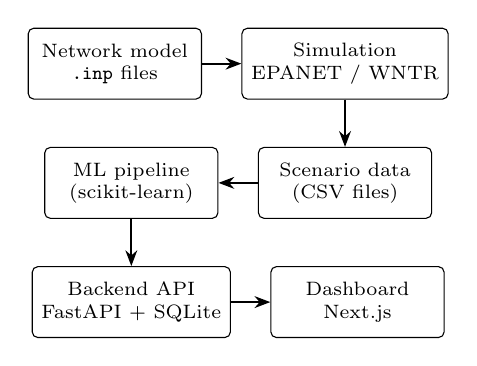
\begin{tikzpicture}[node distance=5mm,
 box/.style={draw,rounded corners=2pt,minimum width=2.2cm,minimum height=0.9cm,align=center,font=\scriptsize},
 arr/.style={-{Stealth[length=2mm]},thick}]
\node[box](a){Network model\\ \texttt{.inp} files};
\node[box,right=of a](b){Simulation\\ EPANET / WNTR};
\node[box,below=6mm of b](c){Scenario data\\ (CSV files)};
\node[box,left=of c](d){ML pipeline\\ (scikit-learn)};
\node[box,below=6mm of d](e){Backend API\\ FastAPI + SQLite};
\node[box,right=of e](f){Dashboard\\ Next.js};
\draw[arr](a)--(b);\draw[arr](b)--(c);\draw[arr](c)--(d);\draw[arr](d)--(e);\draw[arr](e)--(f);
\end{tikzpicture}
\caption{End-to-end architecture, from network models to the user's screen.}\label{fig:arch}
\end{figure}
The code is organised as a monorepo: \code{simulation/} builds scenarios and runs the simulator, \code{ml\_pipeline/} holds data loading, features, detector, classifier, localizer and evaluation, \code{backend/} exposes the results, \code{frontend/} is the dashboard and \code{data/} holds networks, simulated scenarios and result files.

\section{Technologies and Their Roles}
\begin{table}[H]
\centering\small
\caption{Technologies used.}\label{tab:tech}
\begin{tabularx}{\textwidth}{@{}p{1.25in}Y@{}}
\toprule
Technology & Role \\
\midrule
EPANET 2.2, WNTR 1.5 & Network files; simulation of every scenario with pressure-dependent demand \\
Python, pandas, NumPy & Data tables and numerical computation \\
NetworkX & Pipe graph, shortest paths (hops, metres) and neighbours (search region) \\
scikit-learn 1.9, joblib & Random forest and decision tree; evaluation metrics; saving the model \\
FastAPI, Uvicorn, Pydantic & REST endpoints and validated response schemas \\
SQLAlchemy, SQLite & Scenario catalogue (kind, node, size, train/test tag) \\
Next.js 16, React 19, TypeScript & The dashboard \\
Tailwind CSS 4 & Styling with colour tokens for light and dark themes \\
React Flow, Recharts, lucide-react, axios & Network map, charts, icons and API calls \\
\bottomrule
\end{tabularx}
\end{table}

\section{Backend and Database}
The backend creates an SQLite table \texttt{scenarios} at start-up from the generated files, so the dashboard always lists exactly what exists. Its columns are the scenario identifier, network, name, group, kind, true leak nodes, a JSON field of parameters (kind, node, size, noise, hidden-by, train/test tag) and the data folder. The time series stay in CSV files. Scenario identifiers are validated against a whitelist of characters before any file is read.
\begin{table}[H]
\centering\small
\caption{Backend endpoints.}\label{tab:api}
\begin{tabularx}{\textwidth}{@{}p{2.0in}Y@{}}
\toprule
Endpoint & Returns \\
\midrule
\texttt{GET /api/networks} & Networks with junction and scenario counts \\
\texttt{GET /api/scenarios?network=} & Scenario list with parameters and train/test tag \\
\texttt{GET /api/network?network=} & Node positions and pipes for the map \\
\texttt{GET /api/analyze/\{id\}} & Verdict, probabilities, features, ranked nodes, search region, affected nodes, per-node and per-pipe numbers, true answer \\
\texttt{GET /api/evaluation} & The saved test results \\
\bottomrule
\end{tabularx}
\end{table}
When the dashboard requests an analysis, the backend loads the saved tables of the scenario and the baseline, runs the analysis of Section~5.9 (about 22 ms), and returns one JSON object. The simulation is \emph{not} run at that time: it was run beforehand and its results were saved.

\section{The Dashboard}
The first prototype exposed two long drop-down lists and technical vocabulary. The redesigned dashboard, named LeakLens, follows these principles.
\begin{itemize}
\item \textbf{Guided choice:} three steps (network, what happened, narrow it down) with a counter of matching scenarios, node search and \emph{Pick on map}, size and condition filters, and next/previous and random-scenario buttons.
\item \textbf{Plain-language verdict:} a headline, a confidence label, a ``what to do'' sentence and reasons written from the measurements. The reasons are fixed templates that appear when a feature passes a limit (for example, a pump-flow loss above 0.5 or an unaccounted-flow ratio of at least 1).
\item \textbf{Honest testing built in:} every scenario carries an \emph{Unseen test} or \emph{Training} tag, unseen scenarios are shown by default, and analysing a training scenario shows a warning that a correct answer proves little.
\item \textbf{Explained terms, themes and accessibility:} dotted-underline words show definitions, light and dark themes follow the system setting, controls are labelled and keyboard accessible, and the layout adapts to phones.
\item \textbf{Performance and Guide tabs:} the test results of Chapter~7 in plain language, and a glossary.
\end{itemize}
\begin{figure}[H]
\centering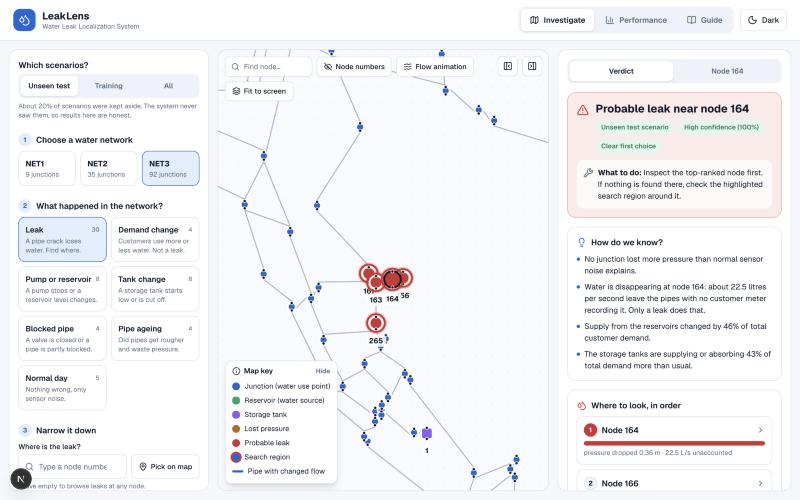
\includegraphics[width=\textwidth]{figures/ui_light_leak.jpg}
\caption{The Investigate screen (light theme) after analysing a leak: choose a scenario on the left, the network map in the centre, the verdict and reasons on the right.}\label{fig:ui1}
\end{figure}
\begin{figure}[H]
\centering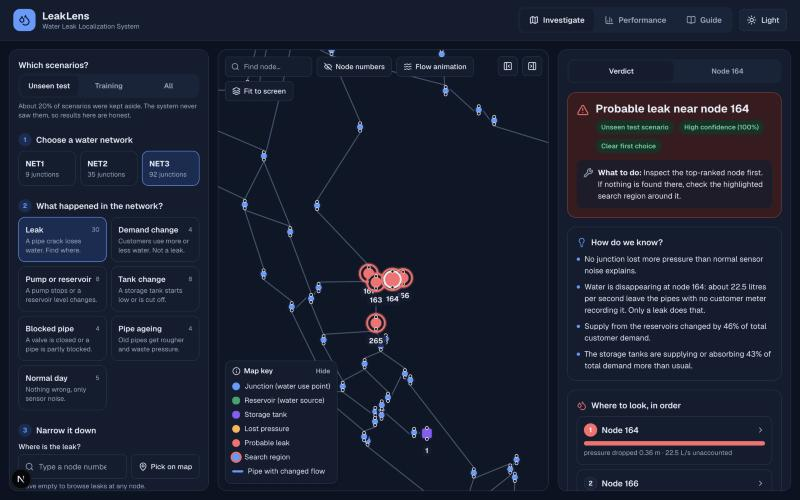
\includegraphics[width=\textwidth]{figures/ui_dark_leak.jpg}
\caption{The same screen in the dark theme, with the predicted node and its search region.}\label{fig:ui2}
\end{figure}

\section{Reproducibility}
The scenarios, the split and the model are generated by scripts with fixed random seeds, in the order: \code{build\_scenarios.py}, \code{generate\_dataset.py}, \code{train.py}, \code{evaluate.py}; the backend and the dashboard are then started with \code{uvicorn main:app} and \code{npm run dev}. Re-training on the same rows reproduces the same forest.

%% ================================================================ CHAPTER 7
\chapter{Experimental Evaluation}
\section{Training and Test Protocol}
\begin{definition}[Hold-out split]\label{def:split}
All scenarios are split once (random seed 42) into a \emph{training set} (about 80\%) used for learning, and a \emph{test set} (about 20\%) used only for measuring performance. Scenarios that are near-copies stay on the same side: all leaks at one junction (every size, start time, noise level and ``hidden-behind'' variant), and a scenario with its sensor-noise twin. The split is stratified by network and kind of event.
\end{definition}
\begin{table}[H]
\centering\small
\caption{Training and test scenarios by kind of event.}\label{tab:split}
\centering\setlength{\tabcolsep}{4pt}
\begin{tabular}{@{}lrrr@{}}
\toprule
Kind of event & All & Train & Test \\
\midrule
Normal day & 54 & 42 & 12 \\
Leak & 299 & 232 & 67 \\
Demand change & 60 & 48 & 12 \\
Pump / reservoir & 54 & 42 & 12 \\
Tank change & 60 & 48 & 12 \\
Blocked pipe & 48 & 36 & 12 \\
Pipe ageing & 42 & 30 & 12 \\
\midrule
Total & 617 & 478 & 139 \\
\bottomrule
\end{tabular}
\end{table}
The noise thresholds and the random forest are fitted on the 478 training scenarios only, and every result below is measured on the 139 test scenarios. Because groups of near-copies are kept together, the share is 77.5\% and 22.5\%, not exactly 80\% and 20\%. The ranking weight (0.3) and the quiet-check cut-offs were chosen during development while looking at all scenarios, before the split existed, and were not re-tuned.

\section{Evaluation Metrics}
\paragraph{Detection.} A scenario is positive if any abnormal event happened. With true positives (TP), false positives (FP), false negatives (FN) and true negatives (TN),
\begin{align}
\text{precision}&=\frac{TP}{TP+FP}, & \text{recall}&=\frac{TP}{TP+FN},\\
F_1&=\frac{2\,\text{precision}\cdot\text{recall}}{\text{precision}+\text{recall}}, & \text{false-alarm rate}&=\frac{FP}{FP+TN}.
\end{align}
\paragraph{Classification.} Accuracy is the share of correct answers; per-kind precision, recall and $F_1$ are computed with TP the diagonal of the confusion matrix, FP the column total minus TP and FN the row total minus TP; macro-$F_1$ is the plain average of the seven $F_1$ values.
\paragraph{Localization.} For a test leak with true node $n_s$ let $r_s$ be its position in the sorted list. Then
\begin{equation}
\text{Top-}k=\frac1N\sum_{s=1}^N\mathbf 1[r_s\le k],\qquad \text{mean hops}=\frac1N\sum_{s=1}^N\operatorname{hops}(\hat n_s,n_s).
\end{equation}
\emph{End-to-end} success counts a leak only if the verdict is leak and $r_s=1$.

\section{Detection Results}
\begin{table}[H]
\centering\small
\caption{Detection on the 139 test scenarios (12 normal days).}\label{tab:det}
\centering\footnotesize\setlength{\tabcolsep}{4pt}
\begin{tabular}{@{}lccccrrrr@{}}
\toprule
Detector & Precision & Recall & $F_1$ & False alarms & TP & FP & FN & TN \\
\midrule
Fixed 0.5\,m alarm & 95.7\% & 87.4\% & 91.4\% & 41.7\% & 111 & 5 & 16 & 7 \\
Learned pressure threshold & 100.0\% & 77.2\% & 87.1\% & 0.0\% & 98 & 0 & 29 & 12 \\
Full system & 100.0\% & 93.7\% & 96.7\% & 0.0\% & 119 & 0 & 8 & 12 \\
\bottomrule
\end{tabular}
\end{table}
The full system has precision 100.0\%, recall 93.7\% and $F_1$ 96.7\% with a false-alarm rate of 0.0\%, against 41.7\% for the fixed 0.5~m alarm. With only 12 normal test days the true false-alarm rate is not exactly zero.

\section{Cause Classification Results}
Accuracy on the test scenarios is \textbf{82.7\%} (115 of 139); on the training scenarios it is 95.6\%. The macro-$F_1$ is 76.4\%.
\begin{table}[H]
\centering\small
\caption{Per-kind precision, recall and $F_1$ on the test scenarios.}\label{tab:perclass}
\centering\setlength{\tabcolsep}{4pt}
\begin{tabular}{@{}lrrrccc@{}}
\toprule
Kind & TP & FP & FN & Precision & Recall & $F_1$ \\
\midrule
Normal day & 12 & 8 & 0 & 60.0\% & 100.0\% & 75.0\% \\
Leak & 60 & 1 & 7 & 98.4\% & 89.6\% & 93.8\% \\
Demand change & 12 & 0 & 0 & 100.0\% & 100.0\% & 100.0\% \\
Pump / reservoir & 8 & 4 & 4 & 66.7\% & 66.7\% & 66.7\% \\
Tank change & 8 & 6 & 4 & 57.1\% & 66.7\% & 61.5\% \\
Blocked pipe & 9 & 0 & 3 & 100.0\% & 75.0\% & 85.7\% \\
Pipe ageing & 6 & 5 & 6 & 54.5\% & 50.0\% & 52.2\% \\
\bottomrule
\end{tabular}
\end{table}
\begin{table}[H]
\centering\footnotesize
\caption{Confusion matrix on the test scenarios (rows: truth; columns: system; a dot is 0).}\label{tab:conf}
\centering\footnotesize\setlength{\tabcolsep}{4pt}
\begin{tabular}{@{}lrrrrrrrr@{}}
\toprule
Truth $\backslash$ system & Normal & Leak & Demand & Pump & Tank & Blocked & Ageing & Total \\
\midrule
Normal day & 12 & . & . & . & . & . & . & 12 \\
Leak & 6 & 60 & . & . & 1 & . & . & 67 \\
Demand change & . & . & 12 & . & . & . & . & 12 \\
Pump / reservoir & 2 & . & . & 8 & 2 & . & . & 12 \\
Tank change & . & . & . & . & 8 & . & 4 & 12 \\
Blocked pipe & . & 1 & . & . & 1 & 9 & 1 & 12 \\
Pipe ageing & . & . & . & 4 & 2 & . & 6 & 12 \\
\bottomrule
\end{tabular}
\end{table}
\begin{figure}[H]
\centering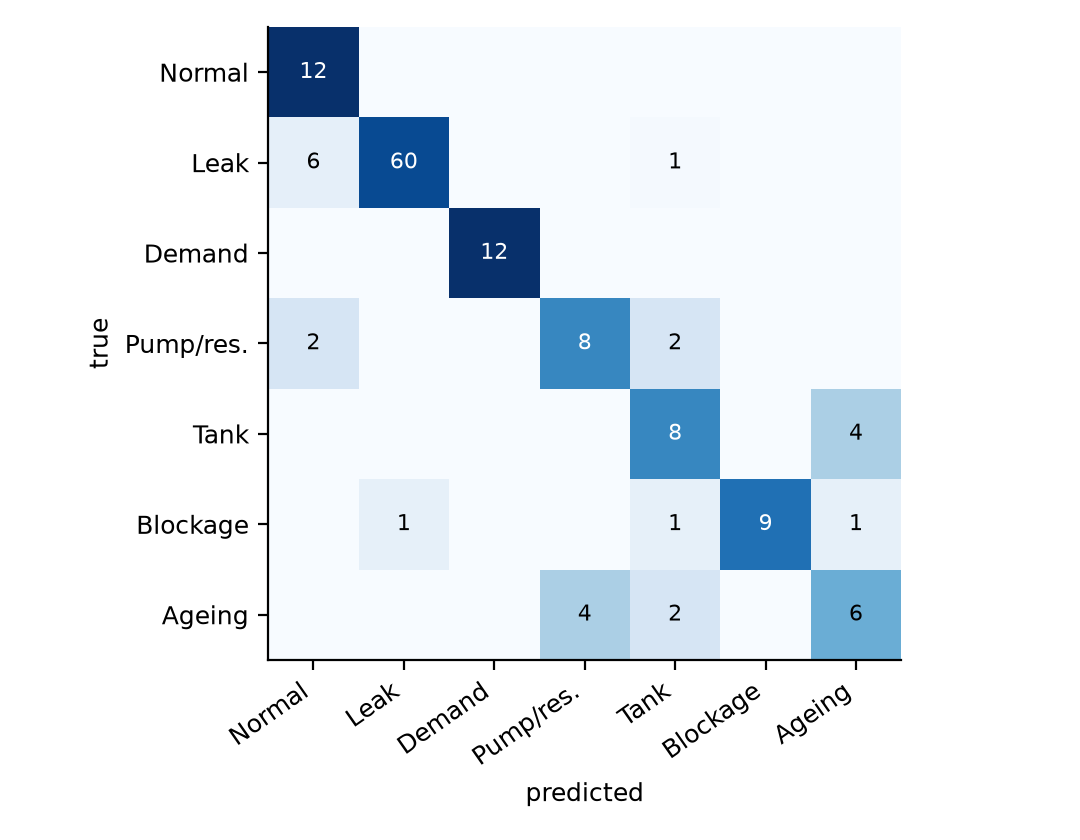
\includegraphics[width=0.62\textwidth]{figures/fig_confusion.png}
\caption{The confusion matrix as a picture.}\label{fig:conf}
\end{figure}
Leaks and demand changes are recognised reliably. Pump, tank, blockage and ageing events are sometimes mistaken for each other, because each lowers pressure over a wide area without losing water. The leak recall is 89.6\%; all seven test leaks that were not named leaks are at Net3 node 601, an ignored pump-outlet node, and only 1.4\% of non-leak events were wrongly called a leak.

\section{Localization Results}
\begin{table}[H]
\centering\small
\caption{Leak localization on the 60 scored test leaks.}\label{tab:loc}
\centering\footnotesize\setlength{\tabcolsep}{4pt}
\begin{tabular}{@{}lcccccc@{}}
\toprule
Method & Top-1 & Top-3 & Top-5 & Mean hops & $\leq1$ hop & Metres \\
\midrule
First prototype & 58.3\% & 70.0\% & 71.7\% & 3.35 & 58.3\% & 1774 \\
\textbf{Final method} & 96.7\% & 98.3\% & 98.3\% & 0.13 & 96.7\% & 60 \\
Final + smoothing & 96.7\% & 98.3\% & 98.3\% & 0.13 & 96.7\% & 60 \\
Final, no demand meters & 93.3\% & 98.3\% & 98.3\% & 0.72 & 93.3\% & 303 \\
Pressure only & 60.0\% & 70.0\% & 70.0\% & 3.05 & 61.7\% & 1208 \\
Pressure only + smoothing & 50.0\% & 63.3\% & 65.0\% & 3.18 & 58.3\% & 1244 \\
\bottomrule
\end{tabular}
\end{table}
\begin{figure}[H]
\centering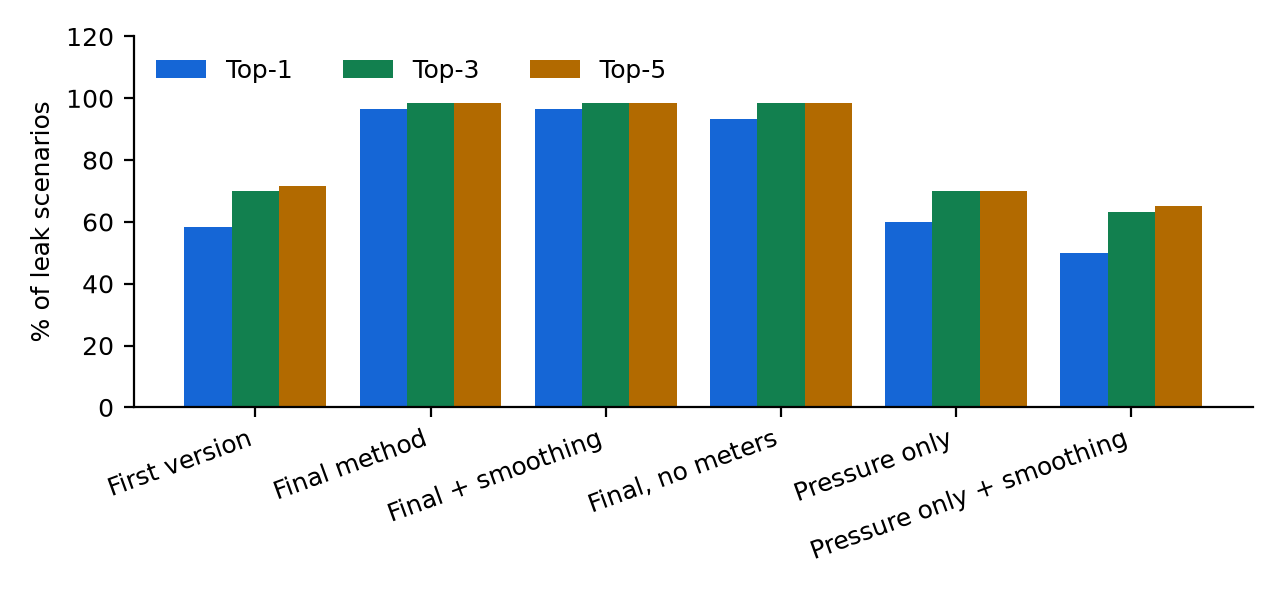
\includegraphics[width=0.85\textwidth]{figures/fig_localization.png}
\caption{Top-1, Top-3 and Top-5 of each localization method on the test leaks.}\label{fig:loc}
\end{figure}
The exact node is ranked first for 58 of 60 test leaks (96.7\%), against 35 of 60 (58.3\%) for the first prototype. The final method is on average 0.13 pipes (about 60~m) from the true node and 96.7\% of the leaks are found at the node or its direct neighbour; end-to-end success is 96.7\%. Without demand meters the Top-1 is 93.3\%, with pressure alone it is 60.0\%, and neighbour smoothing gives 96.7\%. With only 60 test leaks, one miss changes a percentage by about 1.7 points.
\begin{table}[H]
\centering\small
\caption{Top-1 and Top-5 by leak type, node type and network (final method).}\label{tab:groups}
\centering\setlength{\tabcolsep}{4pt}
\begin{tabular}{@{}lrrrr@{}}
\toprule
Group & Leaks & Top-1 & Top-5 & Mean hops \\
\midrule
Hidden behind another event & 10 & 100.0\% & 100.0\% & 0.00 \\
With sensor noise & 4 & 100.0\% & 100.0\% & 0.00 \\
Size variations & 20 & 90.0\% & 95.0\% & 0.40 \\
Start-time variations & 4 & 100.0\% & 100.0\% & 0.00 \\
Leak at a junction & 22 & 100.0\% & 100.0\% & 0.00 \\
\midrule
Dead End & 17 & 100.0\% & 100.0\% & 0.00 \\
Hub & 1 & 100.0\% & 100.0\% & 0.00 \\
Inline & 42 & 95.2\% & 97.6\% & 0.19 \\
NET1 & 11 & 100.0\% & 100.0\% & 0.00 \\
NET2 & 26 & 92.3\% & 96.2\% & 0.31 \\
NET3 & 23 & 100.0\% & 100.0\% & 0.00 \\
\bottomrule
\end{tabular}
\end{table}

\section{Effect of Leak Size}
\begin{table}[H]
\centering\small
\caption{Effect of hole area on the test leaks.}\label{tab:size}
\centering\footnotesize\setlength{\tabcolsep}{4pt}
\begin{tabular}{@{}crcccc@{}}
\toprule
Area (m$^2$) & Leaks & Noticed by pressure & Called a leak & Top-1 & Top-5 \\
\midrule
0.0001 & 4 & 75.0\% & 100.0\% & 100.0\% & 100.0\% \\
0.0003 & 4 & 100.0\% & 100.0\% & 100.0\% & 100.0\% \\
0.001 & 4 & 100.0\% & 100.0\% & 100.0\% & 100.0\% \\
0.003 & 4 & 100.0\% & 100.0\% & 100.0\% & 100.0\% \\
0.01 & 4 & 100.0\% & 100.0\% & 50.0\% & 75.0\% \\
\bottomrule
\end{tabular}
\end{table}
\begin{figure}[H]
\centering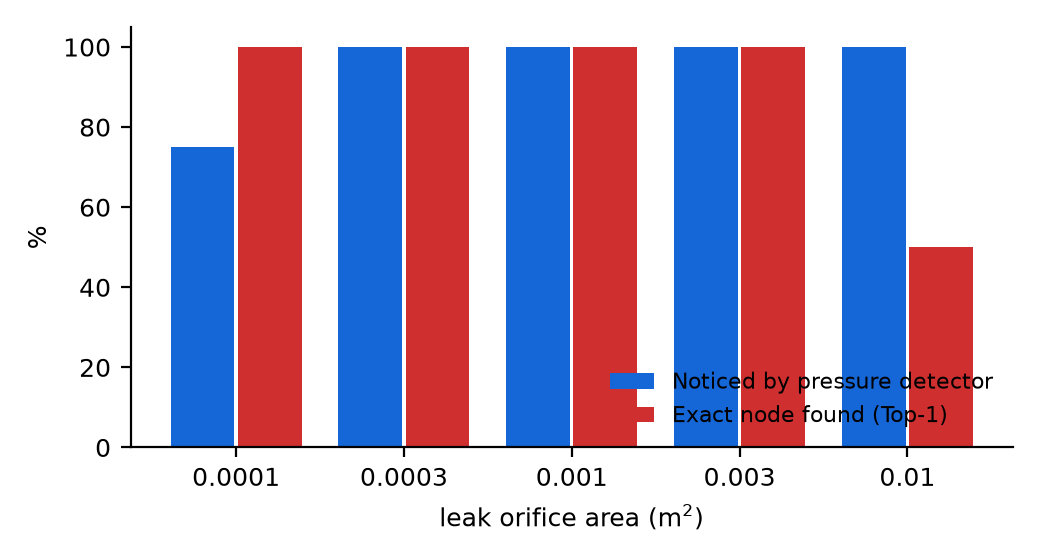
\includegraphics[width=0.62\textwidth]{figures/fig_size.png}
\caption{Detection and exact-node success by leak size.}\label{fig:size}
\end{figure}
Very small leaks sit close to the sensor noise, and the largest leak lowers pressure across the whole network, so its exact node is the hardest to pick. There are only four test leaks per size, so this table is indicative.

\section{A Network Not Seen in Training}
The classifier is trained on the training scenarios of two networks and tested on the test scenarios of the third (leave-one-network-out).
\begin{table}[H]
\centering\small
\caption{Leave-one-network-out results.}\label{tab:lono}
\centering\footnotesize\setlength{\tabcolsep}{4pt}
\begin{tabular}{@{}lrcccc@{}}
\toprule
Unseen network & Test scen. & Accuracy & Leak recall & Leak precision & Accuracy, no meters \\
\midrule
NET1 & 33 & 48.5\% & 100.0\% & 100.0\% & 45.5\% \\
NET2 & 44 & 81.8\% & 92.3\% & 100.0\% & 75.0\% \\
NET3 & 62 & 54.8\% & 73.3\% & 100.0\% & 14.5\% \\
\bottomrule
\end{tabular}
\end{table}
Leaks carry over to a new network, but telling pump, tank, blockage and ageing events apart does not carry over well; without demand meters the accuracy on an unseen Net3 falls to 14.5\%. This is the most important item for Semester~2.

\section{Training Versus Test}
The cause accuracy is 95.6\% on the training scenarios and 82.7\% on the test scenarios, which shows that the forest partly memorises. The leak Top-1 of the ranking is 97.8\% on the 231 training leaks and 96.7\% on the test leaks; the gap is small because the ranking is a fixed formula and is not trained. Table~\ref{tab:history} summarises how the method evolved.
\begin{table}[H]
\centering\small
\caption{Evolution of the method.}\label{tab:history}
\begin{tabularx}{\textwidth}{@{}p{0.65in}YY@{}}
\toprule
Version & Description & Result \\
\midrule
V0 & Fixed 0.5~m alarm; score $=$ pressure drop $+\,50\times$ positive flow divergence & Top-1 58.3\%, false alarms 41.7\% on the test set \\
V1 & Unaccounted flow added; pressure and flow summed in raw units & Top-1 84.9\% (all scenarios): pressure drowned the flow signal \\
V2 & Each signal scaled to 0--1, flow leads, plus neighbour smoothing & Top-1 95.9\% (all scenarios) \\
V3 (final) & As V2 without smoothing & 96.7\% on the unseen test leaks \\
\bottomrule
\end{tabularx}
\end{table}
Two classifier models were compared on the same data: a depth-4 decision tree reaches 69.1\% and the random forest 82.7\% (with the quiet check). We did not test other model families.

\section{Discussion and Limitations}
Unaccounted flow does most of the work: if the customer use at every node is known, water that disappears with no meter behind it is a leak, and a demand change cancels out. This explains the large gain in localization over pressure alone, and why separating demand changes from leaks needs demand data. The following limitations apply.
\begin{itemize}
\item All data are simulated; real networks have model errors and real noise.
\item The test set is small (139 scenarios, 60 scored leaks, 12 normal days) and the split was made once.
\item The ranking weight and the quiet-check cut-offs were chosen before the split and not re-tuned; no hyper-parameter of the forest was tuned.
\item Per-node demand meters are assumed; real utilities usually meter an area and not every node.
\item Leaks inside the sensor noise are called normal; the largest leaks are hard to pinpoint.
\item Pump, tank, blockage and ageing events are confused and do not transfer well to an unseen network.
\item Net3 nodes 61 and 601 and the hour 21:00 are ignored; pump-speed changes were not simulated (the simulator supports only speed 1.0); only single leaks were studied.
\end{itemize}

%% ================================================================ CHAPTER 8
\chapter{Conclusion and Future Work}
\section{Conclusion}
This project built LeakLens, a system that, in simulation, detects abnormal behaviour of a water network without false alarms from sensor noise, names the kind of event, and ranks the junctions where a leak most probably is. On 139 unseen test scenarios the exact leak junction was ranked first for 96.7\% of the test leaks, the cause of an event was named correctly for 82.7\% of the scenarios, and false alarms on normal days fell from 41.7\% to 0.0\%. The key idea, unaccounted flow, is simple and explainable, and the dashboard presents the result in plain language with an honest distinction between training and unseen scenarios.

\section{Future Work}
For Semester~2 we propose:
\begin{itemize}
\item sparse and missing sensors, using graph-based sensor placement \cite{leonzio2026centrality,vangemert2026sensorplacement};
\item estimating demand where nodal meters do not exist;
\item several simultaneous leaks;
\item cause classification that carries over to unseen networks, including graph or algorithm-informed models \cite{zhang2026aignn} compared against this interpretable baseline, and a comparison with gradient boosting \cite{marvin2023hgb};
\item repeated random splits with confidence intervals, and a larger test set;
\item validation on public benchmark data \cite{vrachimis2018leakdb,vrachimis2022battledim} or real utility data.
\end{itemize}

%% ================================================================ REFERENCES
\renewcommand{\bibname}{References}
\clearpage\addcontentsline{toc}{chapter}{References}
\begin{thebibliography}{99}
\bibitem{sousa2026review} A.~L. Sousa, A.~F. Brochado, E. Rocha, and A. Andrade-Campos, ``A state-of-the-art review of scientific, industrial, and commercial developments in water leakage management for water supply systems,'' \textit{Water Research}, vol.~299, 125853, 2026.
\bibitem{romeroben2023review} L. Romero-Ben, D. Alves, J. Blesa, G. Cembrano, V. Puig, and E. Duviella, ``Leak detection and localization in water distribution networks: Review and perspective,'' \textit{Annual Reviews in Control}, vol.~55, pp.~392--419, 2023.
\bibitem{vaquet2024survey} V. Vaquet, F. Hinder, A. Artelt, I. Ashraf, J. Strotherm, J. Vaquet, J. Brinkrolf, and B. Hammer, ``Challenges, methods, data -- a survey of machine learning in water distribution networks,'' in \textit{Artificial Neural Networks and Machine Learning -- ICANN 2024}, 2024.
\bibitem{vrachimis2018leakdb} S.~G. Vrachimis, M.~S. Kyriakou, D.~G. Eliades, and M.~M. Polycarpou, ``LeakDB: A benchmark dataset for leakage diagnosis in water distribution networks,'' in \textit{WDSA/CCWI Joint Conference}, 2018.
\bibitem{vrachimis2022battledim} S.~G. Vrachimis, D.~G. Eliades, R. Taormina, Z. Kapelan, A. Ostfeld, S. Liu, M. Kyriakou, P. Pavlou, M. Qiu, and M.~M. Polycarpou, ``Battle of the leakage detection and isolation methods,'' \textit{Journal of Water Resources Planning and Management}, vol.~148, no.~12, 04022068, 2022.
\bibitem{lucin2021rf} I. Lu\v{c}in, Z. {\v{C}}arija, S. Dru\v{z}eta, and B. Lu\v{c}in, ``Detailed leak localization in water distribution networks using random forest classifier and pipe segmentation,'' \textit{IEEE Access}, vol.~9, pp.~155113--155122, 2021.
\bibitem{marvin2023hgb} G. Marvin, L. Grb\v{c}i\'{c}, S. Dru\v{z}eta, and L. Kranj\v{c}evi\'{c}, ``Water distribution network leak localization with histogram-based gradient boosting,'' \textit{Journal of Hydroinformatics}, 2023.
\bibitem{basnet2023supervised} L. Basnet, D. Brill, R. Ranjithan, and K. Mahinthakumar, ``Supervised machine learning approaches for leak localization in water distribution systems: Impact of complexities of leak characteristics,'' \textit{Journal of Water Resources Planning and Management}, vol.~149, no.~8, 2023.
\bibitem{rajabi2023cdcgan} M.~M. Rajabi, P. Komeilian, X. Wan, and R. Farmani, ``Leak detection and localization in water distribution networks using conditional deep convolutional generative adversarial networks,'' \textit{Water Research}, vol.~238, 120012, 2023.
\bibitem{soldevila2022hybrid} A. Soldevila, G. Boracchi, M. Roveri, S. Tornil-Sin, and V. Puig, ``Leak detection and localization in water distribution networks by combining expert knowledge and data-driven models,'' \textit{Neural Computing and Applications}, vol.~34, no.~6, pp.~4759--4779, 2022.
\bibitem{irofti2021dictionary} P. Irofti, L. Romero-Ben, F. Stoican, and V. Puig, ``Data-driven leak localization in water distribution networks via dictionary learning and graph-based interpolation,'' arXiv:2110.06372, 2021.
\bibitem{leonzio2026centrality} D.~U. Leonzio, T. Cattai, P. Bestagini, S. Colonnese, and S. Tubaro, ``Centrality-guided node selection for efficient water leak detection,'' \textit{IEEE Access}, vol.~14, pp.~24432--24446, 2026.
\bibitem{zhang2026aignn} Z. Zhang and O. Fink, ``Algorithm-informed graph neural networks for leakage detection and localization in water distribution networks,'' \textit{Reliability Engineering \& System Safety}, vol.~265, 111494, 2026.
\bibitem{vangemert2026sensorplacement} J.~J.~H. van Gemert, V. Breschi, D.~R. Yntema, K.~J. Keesman, and M. Lazar, ``The impact of sensor placement on graph-neural-network-based leakage detection,'' arXiv:2603.24076, 2026.
\bibitem{melnikov2025sicams} O. Melnikov, Y. Dorofieiev, Y. Shakhnovskiy, H. Truong, and V. Degeler, ``A multivariate statistical framework for detection, classification and pre-localization of anomalies in water distribution networks,'' arXiv:2512.15685, 2025.
\bibitem{epanet} U.S. Environmental Protection Agency, \textit{EPANET 2.2: Water Distribution System Hydraulic and Water Quality Modeling}.
\bibitem{wntr} U.S. Environmental Protection Agency, \textit{WNTR: Water Network Tool for Resilience}.
\end{thebibliography}

%% ================================================================ APPENDICES
\appendix
\chapter{Decision-Tree Rules}\label{app:rules}
The depth-4 decision tree trained on the training scenarios (file \texttt{decision\_rules.txt}). It is shown only to make the logic readable; the verdict comes from the random forest.
\begin{lstlisting}
|--- unacc_conc <= 0.37
|   |--- demand_frac <= 0.01
|   |   |--- rise_ratio <= 0.94
|   |   |   |--- flow_frac <= 0.09
|   |   |   |   |--- class: normal
|   |   |   |--- flow_frac >  0.09
|   |   |   |   |--- class: valve_block
|   |   |--- rise_ratio >  0.94
|   |   |   |--- conc_drop <= 0.03
|   |   |   |   |--- class: tank_event
|   |   |   |--- conc_drop >  0.03
|   |   |   |   |--- class: ageing
|   |--- demand_frac >  0.01
|   |   |--- unacc_ratio <= 0.48
|   |   |   |--- median_ratio <= 37.92
|   |   |   |   |--- class: demand_change
|   |   |   |--- median_ratio >  37.92
|   |   |   |   |--- class: tank_event
|   |   |--- unacc_ratio >  0.48
|   |   |   |--- conc_drop <= 0.02
|   |   |   |   |--- class: valve_block
|   |   |   |--- conc_drop >  0.02
|   |   |   |   |--- class: normal
|--- unacc_conc >  0.37
|   |--- class: leak
\end{lstlisting}

\chapter{Example of an Analysis Response}
Abridged response of \texttt{GET /api/analyze/net3\_leak\_15}.
\begin{lstlisting}
{ "network": "net3", "split": "test", "event_class": "leak",
  "probabilities": {"leak": 0.94, ...},
  "predicted_leaks": [{"node_id": "15", "confidence_score": 1.3,
                       "pressure_drop": 6.69, "flow_divergence": 0.0199}, ...],
  "candidate_region": ["143", "15"],
  "scenario_truth": {"event_class": "leak", "leak_nodes": "15"},
  "localization_error_hops": 0 }
\end{lstlisting}

\end{document}
